\section{Appendix: Derivations}

\subsection{Derivation of {\boldmath $p(b|X)$}}
\label{appdx:b|x}

We determine the form of $p(b| X)$ by integrating
out the parameters $\theta$. From the definitions we have:
%
\begin{align*}
	p(b | X) &= \int p(b , \theta| X, \theta) d\theta = \int p(b | X, \theta) p(\theta | X) d\theta \\
	&=\int p(b | X, \theta) p(\theta) d\theta = \int \prod_{i \in [N] } \phi_{b_i}(x_i; \theta) p(\theta) d\theta \\
	&= \prod_{i \in [N]} \int \frac{\exp(w_{b_i}^T \tilde{x}_i) \prod_{j \in [B]} \Gaussian(w_j; 0, \sigma_\theta^2 I)}{\sum_{k \in [B]} \exp(w_{k}^T \tilde{x}_i)} dw_{1:B}.
\end{align*}
%
The key observation here is that 
the value of the integral is independent
of the value of $b_i \in [B]$ as
the integrand has the same form regardless of $b_i$. This is
because the prior is the same for each $w_j$. 
Therefore, the integral is only a function of $\tilde{x}_i$ and $\sigma_\theta^2$,
which means that, as a function of $b$, $p(b|X)\propto 1$. As
$b$ takes values in $[B]^N$, we necessarily have:
%
\begin{equation}
	p(b | X) = \frac{1}{\big|[B]^N\big|}=B^{-N}.
\end{equation}

\subsection{Derivation of {\boldmath $\;U(\theta)$}}
\label{appdx:form-U}

Recall from~(\ref{eq:U}) in Section~\ref{s:sfb} that,
$$	\pi_\theta(\theta) \propto p(\theta | X, b) \propto p(b | X, \theta) p(\theta) \propto  \exp \left( - U(\theta) \right),
$$ 
so that $U$ can be expressed as,
$$
U(\theta) 
= - \left( \log p(b | X, \theta) + \log p(\theta) \right) + \textrm{const}.
$$
Writing,
$y_{ij} \coloneqq \one \left\{ b_i = j \right\}$ and 
$a_{ij} \coloneqq \phi_j(x_i; \theta)$, we have that,
%
\begin{equation}
	\log p(b | X, \theta) = \sum_{i \in [N]} \sum_{j \in [B]} y_{ij} \log a_{ij}  \quad \textrm{and} \quad
	\log p(\theta) = -\frac{(D+1)(B)}{2} \log 2\pi - \frac{1}{2 \sigma_\theta^2} 
	\|\theta \|^2,
	\label{eqn:U-constituent-terms}
\end{equation}
%
where
$\|\theta\|^2 = \sum_{i} \theta_{i}^2 = \sum_{j \in [B]} \|w_j\|^2$ 
is the Euclidean norm of the vector of parameters $\theta$.
Therefore, discarding constant terms, we 
obtain exactly the representation~(\ref{eqn:U-form}), as claimed.

\subsection{Derivation of {\boldmath $\;\nabla U(\theta)$}}
\label{appdx:gradu}
Here we show how the gradient 
$\nabla U(\theta)$ can be computed explicitly.
Recall the expression for $U(\theta)$ in~(\ref{eqn:U-form}).
Writing $\theta$ as
$\theta = \left[w_1^T, w_2^T \dots w_B^T  \right]^T$,
in order to compute the gradient
$\nabla U(\theta)$ we need to compute
each of its components,
$\nicefrac{\partial U}{\partial w_k}$,
$1\leq k\leq B$.
To that end, we first compute,
%
\begin{align}
	\frac{\partial a_{ij}}{\partial w_k} &= \frac
	{\tilde{x}_i \exp(w_j^T \tilde{x}_i) \delta_{jk} \cdot \sum_{r \in [B]} \exp(w_r^T \tilde{x}_i) 
		- 
		\exp(w_j^T \tilde{x}_i) \cdot \tilde{x}_i \exp(w_k^T \tilde{x}_i)}
	{\left( \sum_{r \in [B]} \exp(w_r^T \tilde{x}_i) \right)^2} \nonumber \\
	&= \tilde{x}_i \left( a_{ij} \delta_{jk} - a_{ij}a_{ik} \right), 
	\label{eq:dadw}
\end{align}
%
where $\delta_{jk} \coloneqq \one \left\{ j = k \right\}$,
and we also easily find,
%
\begin{equation}
	\frac{ \partial}{\partial w_k} \|\theta\|^2 = \frac{\partial}{\partial w_k} \left( \sum_{r \in [B]} \|w_r\|^2 \right) = 2w_k.
	\label{eq:dtsdw}
\end{equation}
%
Using~(\ref{eq:dadw}) and~(\ref{eq:dtsdw}), we obtain,
\begin{align}
	\frac{\partial U}{\partial w_k} &= 
	\sum_{i \in [N]} \sum_{j \in [B]} y_{ij} 
	\left( -\frac{\tilde{x}_i}{a_{ij}} \left( a_{ij} \delta_{jk} - a_{ij} a_{ik} \right) \right)
	+ \frac{w_k}{\sigma_\theta^2} \nonumber \\
	&=  - \left( \sum_{i \in [N]} \tilde{x}_i \left( y_{ik} - a_{ik} \sum_{j \in [B]} y_{ij} \right)
	- \frac{w_k}{\sigma_\theta^2} \right) \nonumber \\
	&= - \left( \sum_{i \in [N]} \Big\{ \tilde{x}_i (y_{ik} - a_{ik}) \Big\} - \frac{w_k}{\sigma_\theta^2} \right).
\end{align}
%
This can be computed 
efficiently through matrix operations. The only property of $y_{ij}$ 
we have used in the derivation is the constraint $\sum_{j \in [B]} y_{ij} = 1$,
for all $i$.

\subsection{Hypothesis test on feature weights}
\label{appdx:hyp-test}

We are given samples $\{\theta^{(t)}\}_{t \in \Tcal_\theta} \sim p(\theta | A, X)$ and wish to determine the statistical significance of the weights. We adopt matrix notation for simplicity by representing $\theta$ with the matrix $B \times D$ matrix of feature weights $W$. The question is to determine the significance of a particular feature $d$ by examining the value of $W_{id}$ for all the values $i \in [B]$. We know that the posterior is proportional to the prior multiplied by the likelihood (assuming that the feature matrix $X$ is already given):
%
\begin{equation}
	p(\theta|A, X) \propto p(\theta) \cdot p(A | \theta, X)
\end{equation}
%
The prior term can be evaluated but the likelihood is intractable. The closest we can get is through a Monte-Carlo integration over $b$:
%
\begin{align}
	p(A | \theta, X) &= \sum_{b \in [B]^N} p(A, b | \theta, X) \nonumber \\
	&= \sum_{b \in [B]^N} p(A | b, \theta, X) \cdot p(b | \theta, X) \nonumber \\
	&= \sum_{b \in [B]^N} p(A | b) \cdot p(b | \theta, X) \nonumber \\
	&\approx \sum_{i} p\left( A | b^{(i)} \right) \quad \textrm{with} \quad b^{(i)} \sim p(b| \theta, X)
	\label{eqn:mc-likelihood}
\end{align}
%
This could be implemented for a single value of $\theta$ but such a form cannot be used to characterise the overall form of the posterior. Nevertheless, the form in equation \ref{eqn:mc-likelihood} still does highlight something interesting. The likelihood is peaked around areas of $\theta$ that generate a partition $b$ that is highly likely in the SBM sense -- high $p(A|b)$. This provides the motivation for using the Laplace approximation for modelling the posterior $p(\theta | A, X) \approx p(\theta; \mu, \Sigma)$. Indeed, the Laplace approximation is often used for modelling the posterior in logistic classification \cite{laplace}. This approximation is not exact but it motivates the derivation of the dimensionality reduction technique we construct by analogy with hypothesis testing. Marginalising over the other elements, the posterior for each element of the weight matrix $W$ can be approximated by:
%
\begin{equation}
	p(W_{ij}|A, X) \approx \Gaussian(W_{ij}|\hat{\mu}_{ij}, \hat{\sigma}_{ij}^2)
\end{equation}
%
Where we have used the set of samples for $W$ drawn according to the exact posterior, to calculate unbiased estimates for the mean and standard deviation:
%
\begin{equation}
	\hat{\mu}_{ij} \coloneqq \frac{1}{|\Tcal_\theta|} \sum_{t \in \Tcal_\theta} W_{ij}^{(t)} \qquad \textrm{and} \qquad
	\hat{\sigma}_{ij}^2 \coloneqq \frac{1}{|\Tcal_\theta|} \sum_{t \in \Tcal_\theta} \left( W_{ij}^{(t)} - \hat{\mu}_{ij} \right)^2
\end{equation}
%
This approximation is not exact but we can show it is accurate empirically. Indeed, if we run the primary school experiment with hyper-parameters given in appendix \ref{appdx:hyperparams}, we can then plot histograms of the collected $W$-samples and compare these to the Laplace approximation. The results are given on figure \ref{fig:school-histogram}. Even though the Laplace approximation is not exact, it is remarkably reliable. 

\begin{figure}[!h]
	\centering
	\begin{subfigure}[t]{0.3\linewidth}
		\centering
		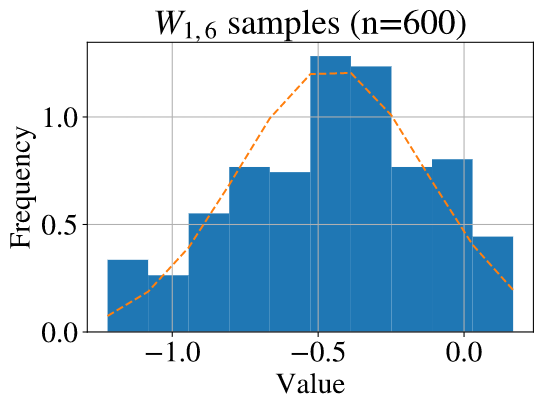
\includegraphics[width=\linewidth]{school-sample-histogram-16.png}
		\caption{Weight for block 1, class 3B}
	\end{subfigure}
	\hfill
	\begin{subfigure}[t]{0.3\linewidth}
		\centering
		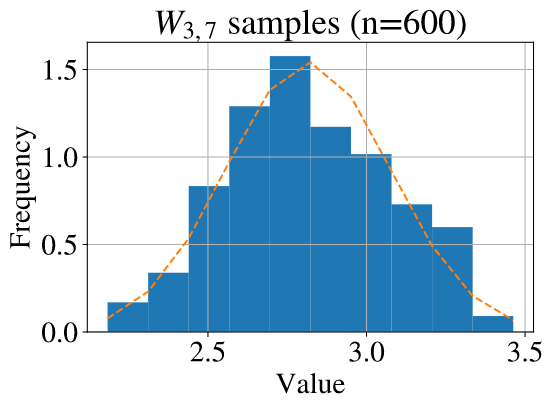
\includegraphics[width=\linewidth]{school-sample-histogram-37.png}
		\caption{Weight for block 3, class 4A}
	\end{subfigure}
	\hfill
	\begin{subfigure}[t]{0.3\linewidth}
		\centering
		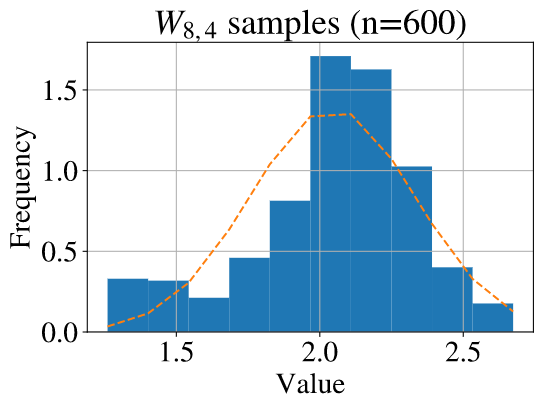
\includegraphics[width=\linewidth]{school-sample-histogram-84.png}
		\caption{Weight for block 8, class 2B}
	\end{subfigure}

	\caption{Histograms of sampled weights for the primary school experiment \cite{schools}. Dotted line is the applied Laplace approximation.}
	\label{fig:school-histogram}
\end{figure}

Using the approximation, we wish to construct a test to determine whether a particular weight value has $|W_{ij}| > c$ with high probability, where $c>0$. More specifically, we wish to determine:
%
\begin{equation}
	\begin{aligned}
		H_0&: |W_{ij}| \leq c \\
		H_1&: |W_{ij}| > c
	\end{aligned}
\end{equation}
%
We can consider the probabilities $p(W_{ij} > c)$ and $p(W_{ij} < c)$ separately. Starting with $p(W_{ij} > c)$ we can write:
%
\begin{align*}
	p(W_{ij} > c) &= p\left(Z > \frac{c - \hat{\mu}_{ij}}{\hat{\sigma}_{ij}}\right) \\
	&= p\left(-Z < \frac{\hat{\mu}_{ij} - c}{\hat{\sigma}_{ij}}\right)\\
	&= \Phi\left(\frac{\hat{\mu}_{ij} - c}{\hat{\sigma}_{ij}}\right)
\end{align*}
%
Where $Z \sim \Gaussian(0,1)$ was introduced as a temporary variable and $\Phi(\cdot)$ is the standard Gaussian cdf. Now we introduce the variable $k$ to control the degree of significance of the result. By enforcing $k$ to be less than the argument of $\Phi$ we show that: 
%
\begin{align*}
	\frac{\hat{\mu}_{ij} - c}{\hat{\sigma}_{ij}} &> k \\
	\hat{\mu}_{ij} - k \hat{\sigma}_{ij} &> c
\end{align*}
%
As $\Phi(\cdot)$ is monotonically increasing, this result gives us that:
%
\begin{equation}
	p(W_{ij} > c) > \Phi(k) \iff \hat{\mu}_{ij} - k \hat{\sigma}_{ij} > c
	\label{eqn:hyp-test-positive}
\end{equation}
%
A similar argument can be made to show that:
%
\begin{equation}
	p(W_{ij} < -c) > \Phi(k) \iff \hat{\mu}_{ij} + k \hat{\sigma}_{ij} < -c
	\label{eqn:hyp-test-negative}
\end{equation}
%
Clearly equations \ref{eqn:hyp-test-positive} and \ref{eqn:hyp-test-negative} cannot both hold simultaneously as $c, \hat{\sigma}_{ij}, k>0$. Nevertheless, a necessary and sufficient condition for one of them to hold is:
%
\begin{equation}
	(\hat{\mu}_{ij} - k \hat{\sigma}_{ij}, \hat{\mu}_{ij} + k \hat{\sigma}_{ij}) \cap (-c, +c) = \emptyset
	\label{eqn:hyp-test-empty}
\end{equation}
%
We therefore choose to reject the null hypothesis $H_0$ if and only if equation \ref{eqn:hyp-test-empty} holds. This tells us with confidence greater than $\Phi(k)$ that either $W_{ij} < -c$ or $W_{ij} > c$ thus rejecting the null $H_0: |W_{ij}| \leq c$. Note that we choose to accept $H_0$ for the case where the combined probabilities of $p(W_{ij} < -c) + p(W_{ij} > c) > \Phi(k)$, if equation \ref{eqn:hyp-test-empty} is not satisfied. This is because we wish to apply this for dimensionality reduction purposes. We only want to keep weights that have a confident prediction outside the null-space not those that succeed by summing the two extremes of their distribution. Note that this case is very rare empirically.